\documentclass[11pt]{article}

\usepackage[letterpaper, margin=1in]{geometry}
\usepackage[utf8]{inputenc}
\usepackage{graphicx}
\usepackage{amsmath}
\usepackage{booktabs}
\usepackage{array}
\usepackage{tabularx}
\usepackage{siunitx}
\usepackage{float}
\usepackage{caption}
\usepackage{subcaption}
\usepackage[version=4]{mhchem}
\usepackage[dvipsnames]{xcolor}
\usepackage{textcomp}
\usepackage{pdfpages}
\usepackage{adjustbox}
\usepackage[numbers,super]{natbib}
\usepackage{fontawesome5}
\usepackage{hyperref}

\graphicspath{{Figures/}{Appendix/}}
\sisetup{detect-all=true, separate-uncertainty=true}
\hypersetup{colorlinks=true, linkcolor=RoyalBlue, citecolor=RoyalBlue, urlcolor=RoyalBlue}
\setlength{\emergencystretch}{2em}

\begin{document}
\begin{center}
    \Large \textbf{Lab \#8: Dipole Moment of Polar Molecules in Solution}
\end{center}
\vspace{0.5em}
\noindent
\begin{minipage}[t]{0.5\textwidth}
    \small
    \textbf{Name:} Yuchen Shi \\
    \textbf{Lab Partner:} Yizhe Dai, Siqi Li \\ 
    \textbf{Section:} 001
\end{minipage}%
\begin{minipage}[t]{0.5\textwidth}
    \small \raggedleft
    \textbf{Date Performed:} 2026-04-21 \\ 
    \textbf{Date Submitted:} 2026-05-05  
\end{minipage}
\vspace{1.5em}

\begin{abstract}
The dipole moment of 1,2-dichlorobenzene in cyclohexane was determined using dielectric-constant and refractive-index measurements of dilute solutions. Dielectric constants were measured with a dielectric constant meter, and refractive indices were measured with a refractometer. Linear fits of $\kappa$, $\rho$, and $n^2$ against solute mole fraction supplied the infinite-dilution parameters used in the Hedestrand and Smith-Guggenheim analyses. The Hedestrand method gave a result of $\mu=(2.3784\pm0.0347)\ \mathrm{D}$, while the Smith-Guggenheim method gave $\mu=(2.3831\pm0.0342)\ \mathrm{D}$. Both values were consistent and slightly lower than the literature value, $2.5000\pm0.0500\ \mathrm{D}$, with percent errors of $4.8649\%$ and $4.6760\%$ respectively. The close agreement between the two methods indicates reliable measurements of the experimental values and analysis methods, while the small negative deviation likely reflects experimental systematic errors.
\end{abstract}

\section*{Introduction}

Molecular polarity is one of the basic physical properties that connects molecular structure with macroscopic behavior. A molecule with an uneven charge distribution has a permanent electric dipole moment, and this dipole moment influences intermolecular interactions, solubility, dielectric behavior, and the way a molecule responds to an external electric field. In solution, however, the dipole moment is not measured by observing one isolated molecule directly. Instead, it must be inferred from bulk properties of the solution. This experiment used that connection between molecular-scale polarity and solution-scale electrical response to determine the dipole moment of 1,2-dichlorobenzene dissolved in cyclohexane.

The solute studied in this experiment was 1,2-dichlorobenzene. It is a polar substituted benzene whose two chlorine atoms are adjacent to one another. Cyclohexane was used as the nonpolar solvent, so changes in the dielectric constant and refractive index could be attributed mainly to the added polar solute. Measurements were made for a series of dilute solutions, and the data were extrapolated to infinite dilution. This infinite-dilution limit is important because it reduces the effect of solute--solute interactions and gives a better estimate of the molecular property of an isolated solute molecule in solution.

Two related analysis methods were used for determination of dipole moment from experimental data. In the Hedestrand method, the dielectric constant and density were fitted as functions of solute mole fraction, and the total molar polarization of the solute was obtained from the limiting slopes and intercepts. The distortion contribution was then estimated from the pure-solute refractive index and density, and subtracted to obtain the orientation polarization. In the Smith-Guggenheim method, the refractive-index data were incorporated directly by fitting $n^2$ as a function of solute mole fraction, allowing the orientation polarization to be calculated from the difference between dielectric and optical polarization terms. Comparing these two methods provided a check on whether the dielectric and refractive-index measurements were internally consistent.

A molecule in an electric field can be polarized in two ways. The electron cloud and nuclei can be distorted, giving an induced or distortion polarization, and a molecule with a permanent dipole moment can partially align with the field, giving an orientation polarization. Thus the molar polarization can be written as
\begin{equation}
P=P_d+P_\mu,
\end{equation}
where $P_d$ is the distortion contribution and $P_\mu$ is the orientation contribution.

In the Hedestrand analysis, the dielectric constant and solution density are fitted as functions of solute mole fraction $X_2$:
\begin{align}
\kappa &= \kappa_1^0+aX_2,\label{eq:kappafit}\\
\rho &= \rho_1^0+bX_2.\label{eq:rhofit}
\end{align}
The infinite-dilution total molar polarization of the solute is then calculated from
\begin{equation}
P_2^0=
\frac{3a}{(\kappa_1^0+2)^2}\frac{M_1}{\rho_1^0}
+
\frac{\kappa_1^0-1}{\kappa_1^0+2}
\left[
\frac{M_2}{\rho_1^0}
-
\frac{M_1b}{(\rho_1^0)^2}
\right].
\label{eq:hedestrand}
\end{equation}
The distortion contribution is estimated from the pure-solute refractive index and density:
\begin{equation}
P_{2,d}^0=
\frac{(n_2^0)^2-1}{(n_2^0)^2+2}\frac{M_2}{\rho_2^0},
\label{eq:distortion}
\end{equation}
so that
\begin{equation}
P_{2,\mu}^0=P_2^0-P_{2,d}^0.
\end{equation}

The Smith-Guggenheim method uses refractive-index data directly. The optical data are fitted as
\begin{equation}
n^2=(n_1^0)^2+cX_2,
\label{eq:nfit}
\end{equation}
and the orientation polarization is calculated from
\begin{equation}
P_{2,\mu}^0=
\frac{3M_1}{\rho_1^0}
\left[
\frac{a}{(\kappa_1^0+2)^2}
-
\frac{c}{((n_1^0)^2+2)^2}
\right].
\label{eq:smith}
\end{equation}
Finally, the dipole moment is obtained from
\begin{equation}
\mu=\sqrt{\frac{9\epsilon_0 kT P_{2,\mu}^0}{N_A}},
\label{eq:dipole}
\end{equation}
where $P_{2,\mu}^0$ must be expressed in $\mathrm{m^3\ mol^{-1}}$. The final value was converted to debye using $1\ \mathrm{D}=3.3356\times10^{-30}\ \mathrm{C\ m}$.

\section*{Experimental}

Four pre-prepared dilute solutions of 1,2-dichlorobenzene in cyclohexane were used. The samples were labeled nominally as 0.010, 0.020, 0.030, and 0.040 M in the lab notebook, while the mole fractions and densities used in the calculations were taken from the calculation guide for the corresponding 1,2-dichlorobenzene solutions. The external lab manual provided necessary experimental measurables for the 1,2-dichlorobenzene solution with specific mole-fraction.\cite{lab_manual}

The dielectric constants were measured first using a dielectric constant meter. The solution cell was filled with the appropriate solution and measurements were made from the lowest to the highest concentration. For each solution, the probe was fully immersed so that the liquid level was above the top of the outer cylinder, and the dielectric constant was read from the instrument display. \cite{lab_manual}

After the dielectric measurements, the same solutions were used for refractive-index measurements with a refractometer. The prism was cleaned and dried before each measurement. 15 drops of solution were placed on the crystal and the prism was cleaned before the next sample. The measured temperatures during the refractive-index measurements were also recorded and used for later calculations, since the dielectric constant is temperature dependent.\cite{lab_manual}

\section*{Results}

\subsection*{Raw data}

The measured dielectric constants, refractive indices, and temperatures are listed in Table~\ref{tab:raw}. The mole fractions and densities are the guide-provided values for 1,2-dichlorobenzene in cyclohexane.\cite{lab_manual}

\begin{table}[H]
\centering
\caption{Experimental data used for dipole-moment analysis. The mole fractions $X_2$ and densities $\rho$ were taken from the calculation guide.}
\label{tab:raw}
\begin{tabular}{cccccc}
\toprule
$X_2$ & $\rho$ / $\mathrm{g\ cm^{-3}}$ & $\kappa$ & $n$ & $n^2$ & $T$ / $^\circ\mathrm{C}$ \\
\midrule
0.010074 & 0.78094 & 2.1000 & 1.4280 & 2.0392 & 19.4000 \\
0.020102 & 0.78640 & 2.1700 & 1.4292 & 2.0426 & 19.6000 \\
0.030180 & 0.79194 & 2.2300 & 1.4306 & 2.0466 & 19.7000 \\
0.040138 & 0.79823 & 2.2900 & 1.4318 & 2.0501 & 19.8000 \\
\bottomrule
\end{tabular}
\end{table}

The average temperature was $\bar T=19.6250^\circ\mathrm{C}=292.7750\ \mathrm{K}$. The sample standard deviation was $s_T=0.1708\ \mathrm{K}$, the standard error of the mean temperature was $s_{\bar T}=0.0854\ \mathrm{K}$, and the 95\% confidence uncertainty was $\lambda=0.2718\ \mathrm{K}$. So the temperature was reported to be $292.7750\pm0.2718K$.

\subsection*{Linear regressions}

The three required linear regressions are shown in Figures~\ref{fig:kappa}--\ref{fig:n2}. The slope and intercept uncertainties shown on the plots are the standard errors from the least-squares regressions. The calculations were done in Python using Numpy\cite{harris2020array} and Matplotlib\cite{Hunter2007} libraries.

\begin{figure}[H]
    \centering
    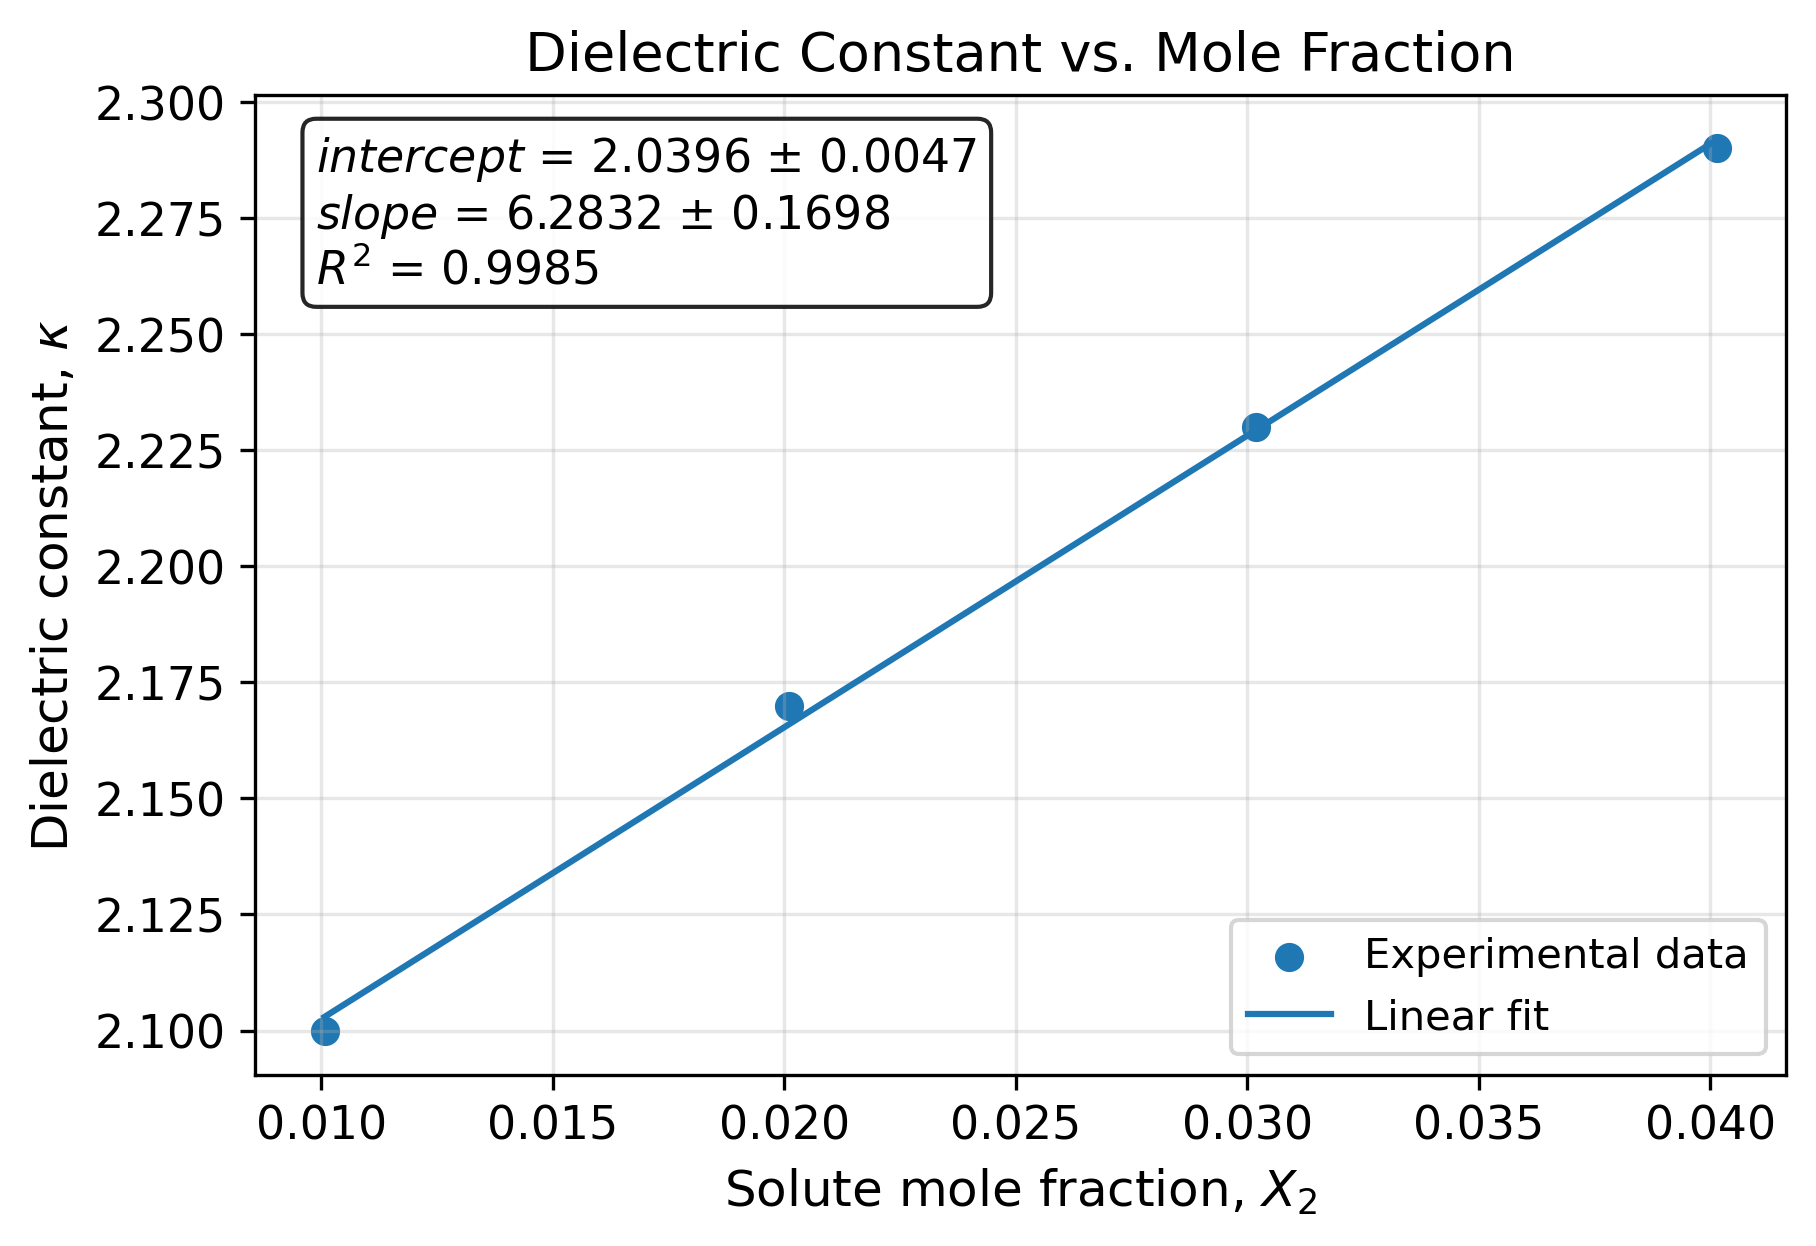
\includegraphics[width=0.75\textwidth]{fig1_kappa_vs_X2.png}
    \caption{Dielectric constant as a function of solute mole fraction. The fit was $\kappa=2.0396+6.2832X_2$, with standard errors shown on the plot.}
    \label{fig:kappa}
\end{figure}

\begin{figure}[H]
    \centering
    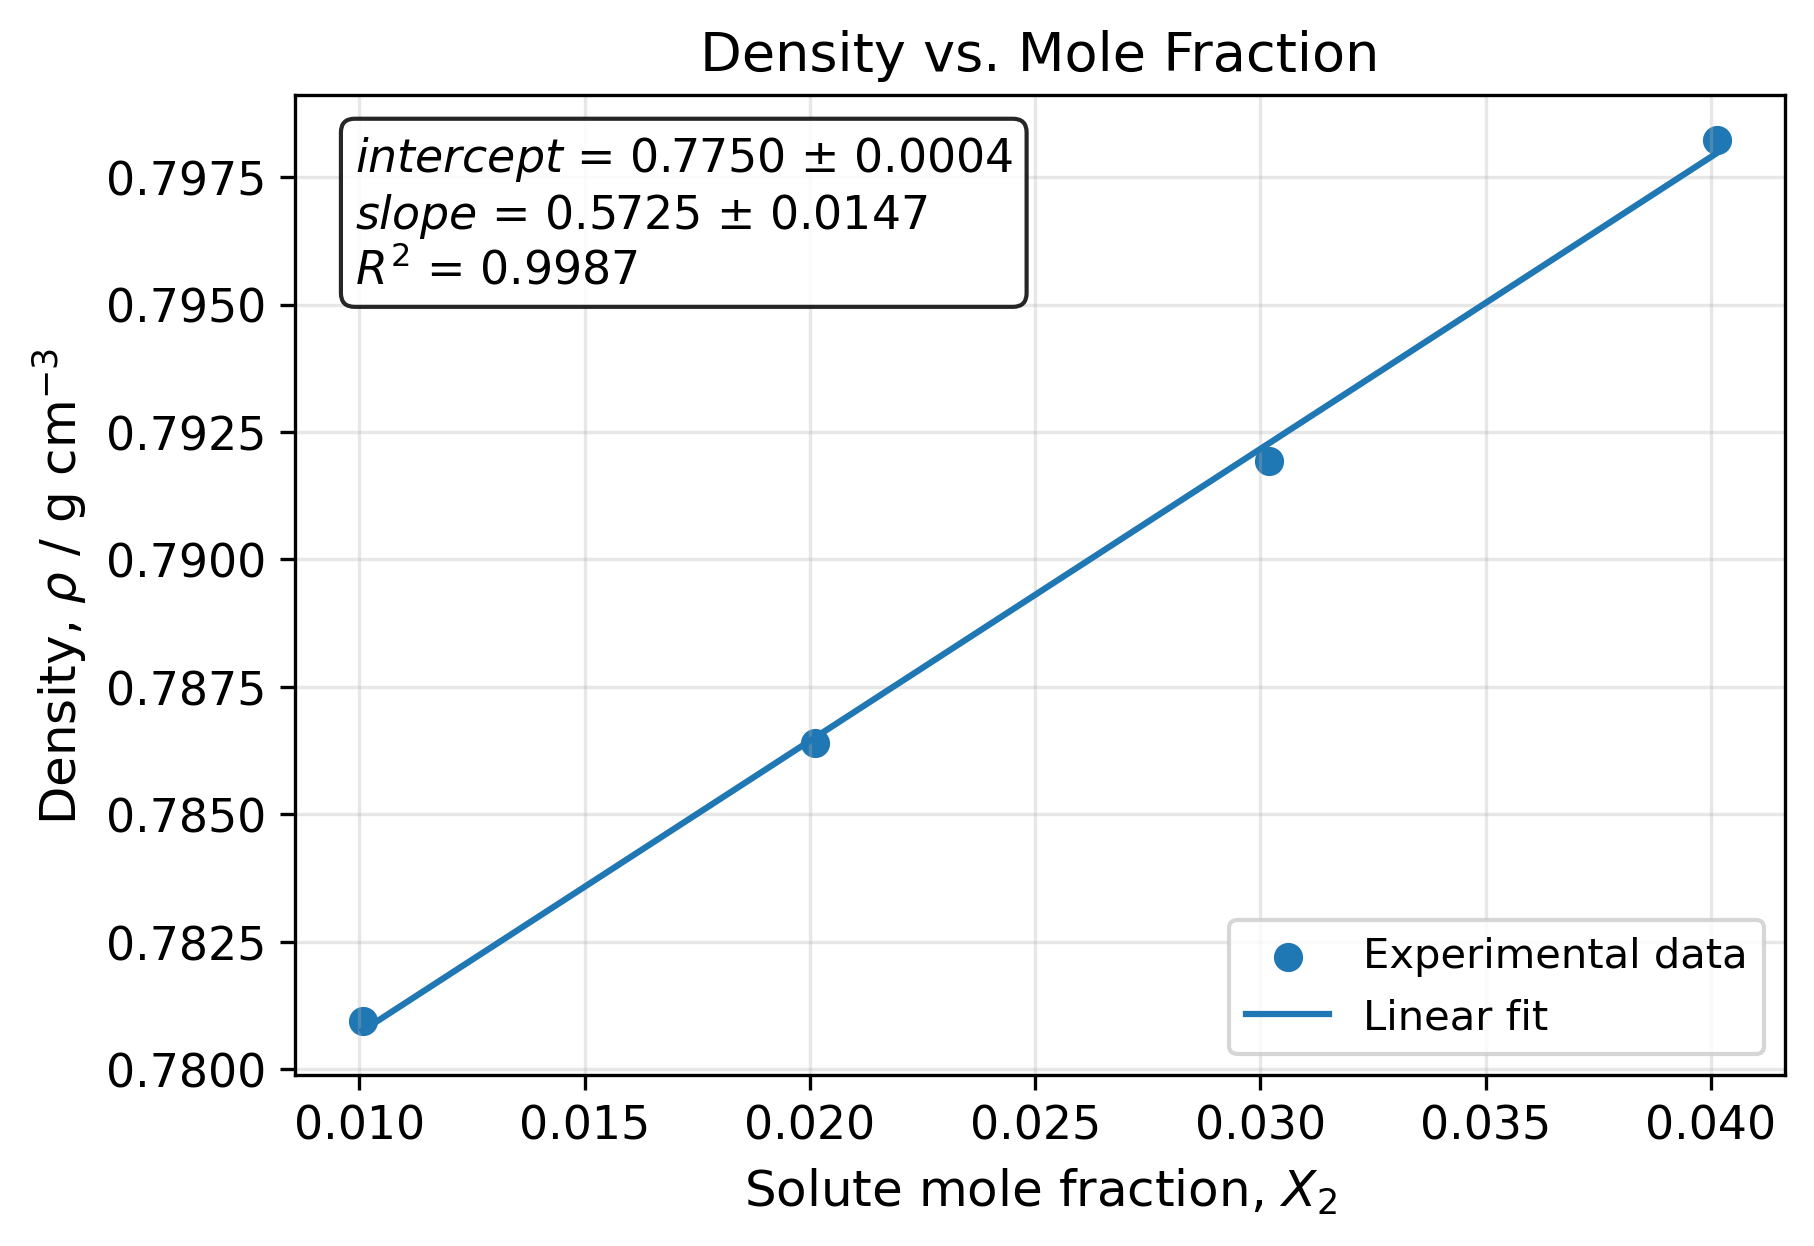
\includegraphics[width=0.75\textwidth]{fig2_density_vs_X2.png}
    \caption{Solution density as a function of solute mole fraction. The fit was $\rho=0.7750+0.5725X_2$, with standard errors shown on the plot.}
    \label{fig:rho}
\end{figure}

\begin{figure}[H]
    \centering
    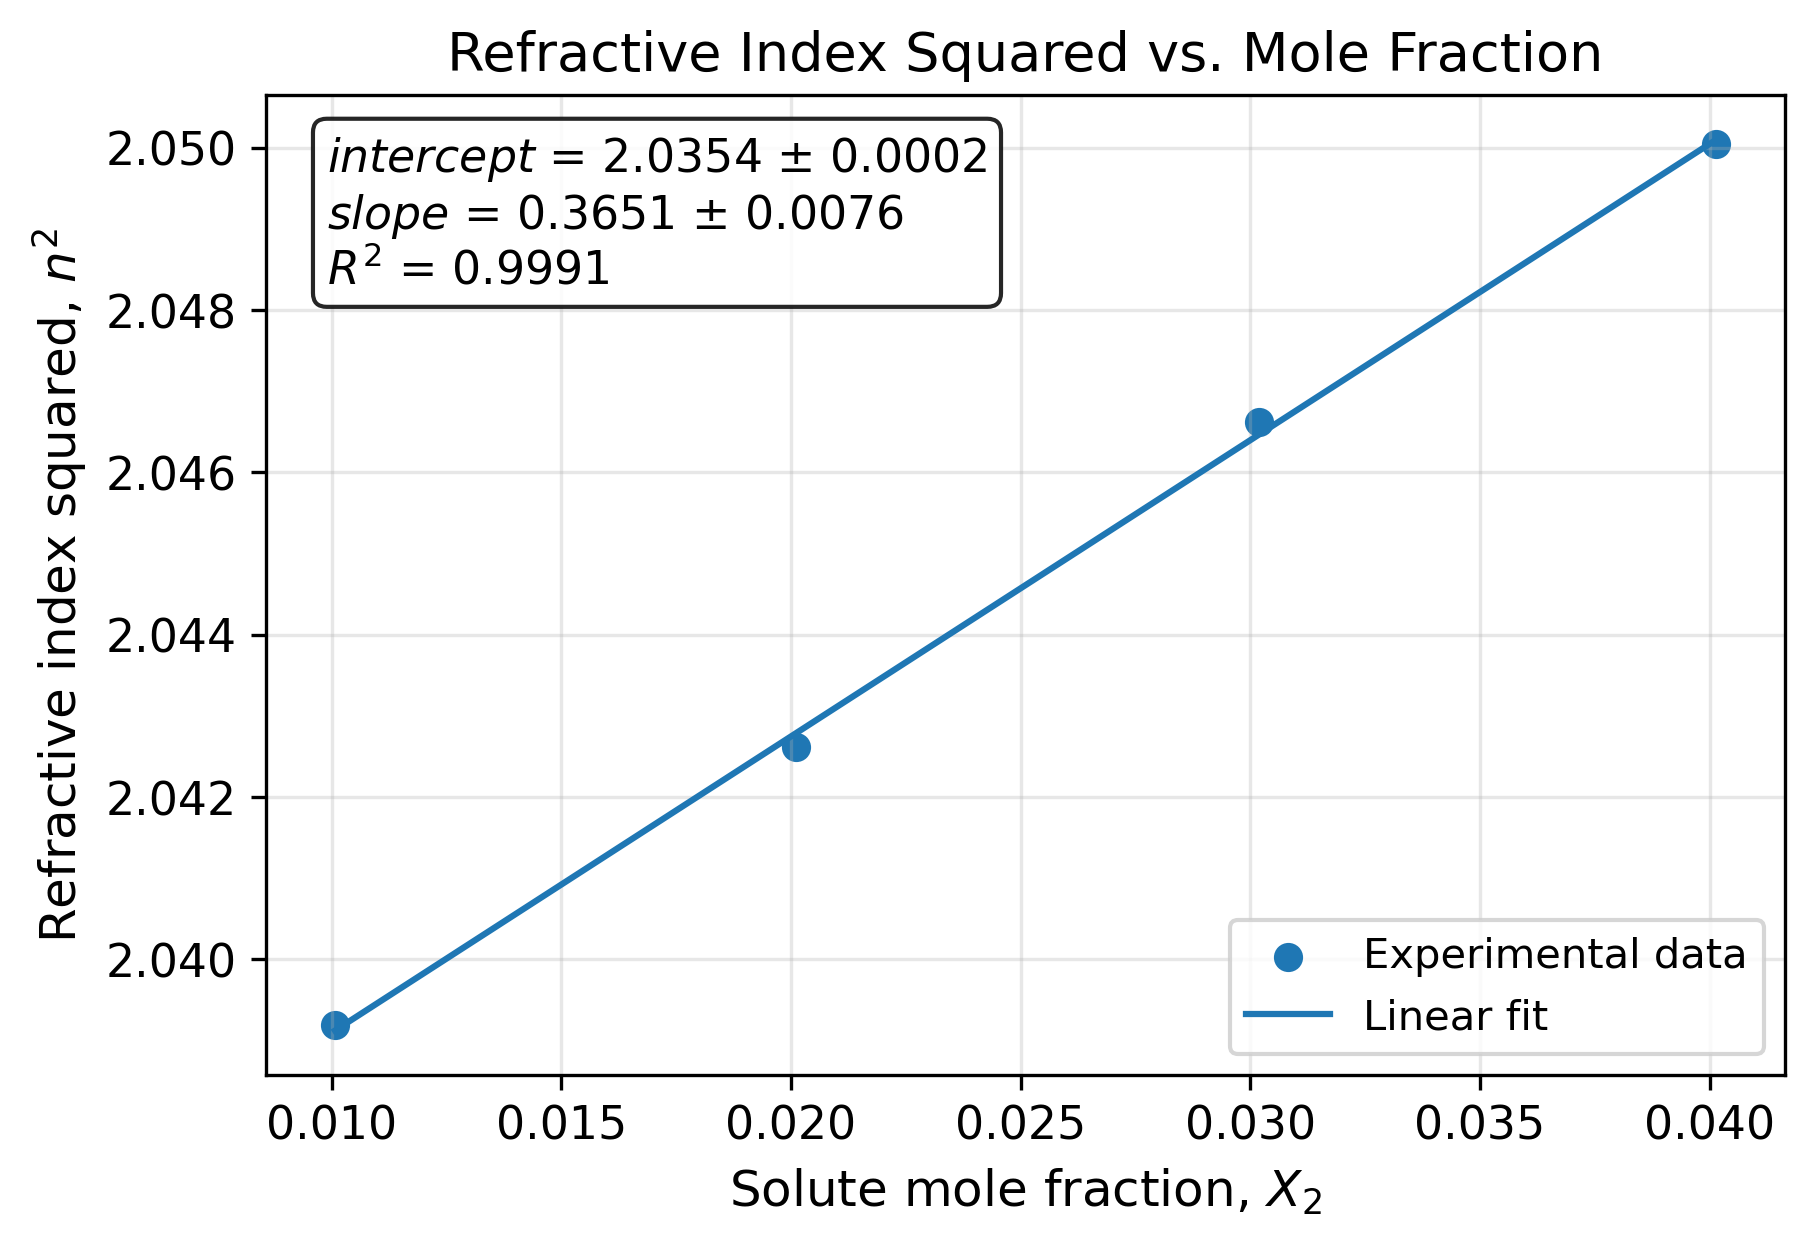
\includegraphics[width=0.75\textwidth]{fig3_n2_vs_X2.png}
    \caption{Refractive index squared as a function of solute mole fraction. The fit was $n^2=2.0354+0.3651X_2$, with standard errors shown on the plot.}
    \label{fig:n2}
\end{figure}

The regression parameters are summarized in Table~\ref{tab:fits}. These fitted values were used in the Hedestrand and Smith-Guggenheim calculations.

\begin{table}[H]
\centering
\caption{Linear regression parameters used in the dipole-moment calculations.}
\label{tab:fits}
\begin{tabular}{lccc}
\toprule
Fit & Intercept & Slope & $R^2$ \\
\midrule
$\kappa$ vs. $X_2$ & $2.0396\pm0.0047$ & $6.2832\pm0.1698$ & 0.9985 \\
$\rho$ vs. $X_2$ & $0.7750\pm0.0004$ & $0.5725\pm0.0147$ & 0.9987 \\
$n^2$ vs. $X_2$ & $2.0354\pm0.0002$ & $0.3651\pm0.0076$ & 0.9991 \\
\bottomrule
\end{tabular}
\end{table}

\subsection*{Calculation summary}

Detailed calculations and error propagation are provided in the handwritten Appendix. 

For the Hedestrand method, Eqs.~\ref{eq:hedestrand}--\ref{eq:dipole} were used with $\kappa_1^0=2.0396$, $a=6.2832$, $\rho_1^0=0.7750\ \mathrm{g\ cm^{-3}}$, and $b=0.5725\ \mathrm{g\ cm^{-3}}$. The pure-solute literature values used for the distortion polarization were $M_2=147.0020\ \mathrm{g\ mol^{-1}}$, $n_2^0=1.5515$, and $\rho_2^0=1.3059\ \mathrm{g\ cm^{-3}}$. The resulting values were $P_2^0=(153.6106\pm3.4312)\ \mathrm{cm^3\ mol^{-1}}$, $P_{2,d}^0=35.9415\ \mathrm{cm^3\ mol^{-1}}$, $P_{2,\mu}^0=(117.6691\pm3.4312)\ \mathrm{cm^3\ mol^{-1}}$, and $\mu=(2.3784\pm0.0347)\ \mathrm{D}$.

For the Smith-Guggenheim method, Eqs.~\ref{eq:smith} and \ref{eq:dipole} were used with $\kappa_1^0=2.0396$, $a=6.2832$, $(n_1^0)^2=2.0354$, and $c=0.3651$. This gave $P_{2,\mu}^0=(118.1368\pm3.3934)\ \mathrm{cm^3\ mol^{-1}}$ and $\mu=(2.3831\pm0.0342)\ \mathrm{D}$. Following the calculation guide, only the uncertainties in $a$ and $b$ were propagated for the Hedestrand $P_2^0$ value, and only the uncertainties in $a$ and $c$ were propagated for the Smith-Guggenheim $P_{2,\mu}^0$ value.\cite{lab_manual}

The literature dipole moment used for comparison was $\mu_{\mathrm{lit}}=(2.5000\pm0.0500)\ \mathrm{D}$ for o-dichlorobenzene.\cite{lide1995crc} The final results and literature comparison are summarized in Table~\ref{tab:final}.

\begin{table}[H]
\centering
\caption{Dipole-moment results and comparison with literature.}
\label{tab:final}
\small
\begin{adjustbox}{max width=\textwidth}
\begin{tabular}{lccccccc}
\toprule
Method & $P_2^0$ & $P_{2,d}^0$ & $P_{2,\mu}^0$ & $\mu$ & $\mu$ & Literature $\mu$ & Error \\
 & \multicolumn{3}{c}{$\mathrm{cm^3\ mol^{-1}}$} & $10^{-30}\ \mathrm{C\,m}$ & D & D & \% \\
\midrule
Hedestrand & $153.6106\pm3.4312$ & 35.9415 & $117.6691\pm3.4312$ & $7.9334\pm0.1157$ & $2.3784\pm0.0347$ & $2.5000\pm0.0500$ & 4.8649 \\
Smith-Guggenheim & -- & -- & $118.1368\pm3.3934$ & $7.9492\pm0.1142$ & $2.3831\pm0.0342$ & $2.5000\pm0.0500$ & 4.6760 \\
\bottomrule
\end{tabular}
\end{adjustbox}
\end{table}


\section*{Discussion}

The three linear regressions were well fitted, with $R^2$ values of 0.9985, 0.9987, and 0.9991. These high $R^2$ values indicate that the dilute-solution data followed the expected linear dependence on solute mole fraction over the concentration range used in this experiment. The fitted intercepts, $\kappa_1^0=2.0396$, $\rho_1^0=0.7750\ \mathrm{g\ cm^{-3}}$, and $(n_1^0)^2=2.0354$, were treated as extrapolated infinite-dilution solvent parameters for the Hedestrand and Smith-Guggenheim calculations. 

Both analysis methods gave nearly the same dipole moment. The Hedestrand method gave $2.3784\pm0.0347\ \mathrm{D}$, while the Smith-Guggenheim method gave $2.3831\pm0.0342\ \mathrm{D}$. The corresponding orientation polarizations also agreed closely: $117.6691\ \mathrm{cm^3\ mol^{-1}}$ from Hedestrand and $118.1368\ \mathrm{cm^3\ mol^{-1}}$ from Smith-Guggenheim. The close agreement indicates that the method of extrapolation had little effect on $P_{2,\mu}^0$ for this data set and that the dielectric-constant and refractive-index data were internally consistent.

The experimental values were both lower than the literature value of $2.5000\pm0.0500\ \mathrm{D}$. The percent errors were $4.8649\%$ for the Hedestrand method and $4.6760\%$ for the Smith-Guggenheim method. Thus, the results are reasonably close to the literature value, but they show a small systematic negative deviation.

The major propagated uncertainty came from the slope of the dielectric-constant fit. This is expected because the orientation polarization is especially sensitive to how strongly $\kappa$ changes with mole fraction. The dielectric constants were recorded only to two decimal places, so small rounding differences in $\kappa$ could noticeably affect the slope $a$. In both the Hedestrand and Smith-Guggenheim uncertainty calculations, the contribution from $a$ was much larger than the contribution from $b$ or $c$.

Several experimental factors could explain the lower experimental dipole moment. The dielectric constant meter probe had to be fully immersed and isolated from the cell walls. Imperfect immersion or contact with the container would affect the dielectric-constant reading. Residual liquid on the probe between samples could also cause carryover between concentrations, even though the procedure required drying the probe with an air compressor. Temperature also mattered because the dielectric constant decreases as temperature increases. The measured temperature range was small, but the solution temperature was still a possible systematic factor. For the refractive-index measurements, any residue left on the prism could also reduce accuracy.

The molecular structure of 1,2-dichlorobenzene is consistent with a nonzero dipole moment. The two C-Cl bond dipoles are adjacent to each other in the ortho isomer, so their vector sum does not cancel. The bond dipoles add to give a net molecular dipole along the approximate bisector of the two C-Cl bonds. This contrasts with the para isomer, where the two C--Cl bond dipoles are approximately opposite and would largely cancel. Therefore, the measured dipole moment near $2.4\ \mathrm{D}$ is chemically reasonable for o-dichlorobenzene.

Overall, the experiment successfully determined the dipole moment of 1,2-dichlorobenzene in cyclohexane. The two independent analysis methods agreed closely, and both gave values within about $5\%$ of the literature value. The most likely limitation of the experiment was the precision of the dielectric-constant measurements, since the dielectric slope controlled most of the propagated uncertainty in the final dipole moment.

\section*{Conclusion}

The dipole moment of 1,2-dichlorobenzene in cyclohexane was determined successfully from dielectric-constant and refractive-index measurements of dilute solutions. Linear extrapolation of $\kappa$, $\rho$, and $n^2$ against solute mole fraction gave the infinite-dilution parameters required for both the Hedestrand and Smith-Guggenheim methods. The Hedestrand method gave $\mu=(2.3784\pm0.0347)\ \mathrm{D}$, and the Smith-Guggenheim method gave $\mu=(2.3831\pm0.0342)\ \mathrm{D}$. The two values showed good internal agreement between the dielectric and optical analyses. Both results were slightly lower than the literature value of $(2.5000\pm0.0500)\ \mathrm{D}$, with percent errors of $4.8649\%$ and $4.6760\%$, respectively. The small negative deviation was most likely caused by limitations in the dielectric-constant measurements, finite-concentration extrapolation, probe or prism residue, and small temperature effects. Overall, the experiment gave a chemically reasonable dipole moment for the ortho isomer, whose adjacent C-Cl bond dipoles produce a nonzero molecular dipole.

\newpage
% References section
% Must follow American Chemical Society (ACS) format.
\bibliographystyle{achemso}
\bibliography{references}


\newpage
\section*{Appendix}
\addcontentsline{toc}{section}{Appendix}
% Include supplementary material (raw output, sample calculations) 
The raw data and corresponding analysis script are available on \href{https://github.com/EasonShi0624/26Spring-PChemLab/tree/main/Lab_8_Dipole_Moment_of_Polar_Molecules_in_Solution}{\textcolor{RoyalBlue}{GitHub} \faGithub}

\begin{figure}[htbp]
    \centering
    
\includegraphics[width=0.7\linewidth, keepaspectratio, page=1]{Lab Computation.pdf}
    \caption{Computations of Values and Error Analysis (Page 1)}
    \label{fig:lab_comp_p1}
\end{figure}

\begin{figure}[htbp]
    \centering
    
\includegraphics[width=0.9\linewidth, keepaspectratio, page=2]{Lab Computation.pdf}
    \caption{Computations of Values and Error Analysis (Page 2)}
    \label{fig:lab_comp_p1}
\end{figure}


\begin{figure}[htbp]
    \centering
    
\includegraphics[width=0.9\linewidth, keepaspectratio, page=3]{Lab Computation.pdf}
    \caption{Computations of Values and Error Analysis (Page 3)}
    \label{fig:lab_comp_p1}
\end{figure}


\begin{figure}[htbp]
    \centering
    
\includegraphics[width=0.9\linewidth, keepaspectratio, page=4]{Lab Computation.pdf}
    \caption{Computations of Values and Error Analysis (Page 4)}
    \label{fig:lab_comp_p1}
\end{figure}


\begin{figure}[htbp]
    \centering
    
\includegraphics[width=0.9\linewidth, keepaspectratio, page=5]{Lab Computation.pdf}
    \caption{Computations of Values and Error Analysis (Page 5)}
    \label{fig:lab_comp_p1}
\end{figure}



\begin{figure}[htbp]
    \centering
    
\includegraphics[width=0.9\linewidth, keepaspectratio, page=1]{lab_note.pdf}
    \caption{Raw Lab Notes}
    \label{fig:lab_notes}
\end{figure}

\end{document}
